\chapter{CHỨC NĂNG TỔNG HỢP CÂU HỎI VÀ TẠO BÀI KIỂM TRA}
\begin{flushleft}
	\fontsize{12pt}{7pt}\selectfont
	\textit{Chương này sẽ trình bày chức năng tổng hợp câu hỏi và tạo bài kiểm tra. Mục đầu tiên sẽ trình bày về thiết kế của iDevice SCORM Quiz được tích hợp sẵn trong hệ thống eXe Learning cùng những ưu, nhược điểm của SCORM Quiz và hướng khắc phục nhược điểm của nó. Mục tiếp theo sẽ trình bày cách thiết kế iDevice SCORM Test, một iDevice có thể tạo bài kiểm tra có các câu hỏi động từ các SCORM Quiz đã có.}
\end{flushleft}

\section{Đặt vấn đề}
\subsection{Chức năng kiểm tra kiến thức hiện tại của eXe Learning}
	Trong việc thiết kế bài học E-Learning, nhu cầu kiểm tra kiến thức của người học sau mỗi bài học là rất cần thiết. Qua đó có thể biết được người học đã tiếp thu được bao nhiêu kiến thức do người soạn thảo trình bày trong bài học. Do đó, cần có một công cụ cung cấp chức năng soạn thảo câu hỏi cho người biên soạn. eXe cung cấp SCORM Quiz với nhiệm vụ và chức năng nói trên.\\

	SCORM Quiz là một trong số các công cụ kiểm tra được thiết kế sẵn trong eXe Learning. Mục đích hướng đến của SCORM Quiz là giúp người soạn thảo có thể biên soạn các câu hỏi ôn tập một cách đơn giản, cho người học biết được số điểm họ làm được sau thi thực hiện xong. Các câu hỏi được biên soạn theo hình thức Mutiple Choice với một câu hỏi và nhiều hơn một lựa chọn, trong đó chỉ có một lựa chọn đúng.\\

	Bên cạnh các ưu điểm kể trên, so với các công cụ kiểm tra có trong các phần mềm soạn thảo bài giảng E-Learning khác thì SCORM Quiz vẫn còn rất nhiều nhược điểm. Sau đây sẽ trình bày về một số ưu điểm cũng như nhược điểm mà SCORM Quiz tồn tại.


\subsection{Nhược điểm của SCORM Quiz }

	Nhược điểm lớn nhất trong thiết kế SCORM Quiz là người biên soạn chỉ có thể thiết lập một SCORM Quiz cho mỗi bài học. Đây là do quan điểm thiết kể của những người phát triển eXe Learning với mỗi bài học sẽ chỉ có được một SCORM Quiz đi cùng. Nhận thấy đây là một thiết kế không linh hoạt với nhu cầu soạn thảo. Nếu như trong một bài học có hai nội dung cần đặt câu hỏi thì với một SCORM Quiz là không đủ.\\
	
	Thứ hai là SCORM Quiz không có thuộc tính phân loại cho các câu hỏi. Về mặt khách quan người soạn thảo sẽ rất khó khăn trong việc đánh giá mức độ của bài trắc nghiệm. Hơn nữa khi người biên soạn xem lại bài học đã soạn thảo từ trước sẽ rất tốn thời gian phân loại và đánh giá.\\
	
	Thứ ba là giao diện soạn thảo câu hỏi khó giao tiếp. Việc soạn thảo câu hỏi của SCORM Quiz được thực hiện trực tiếp trên trình duyệt web, các thao tác với các thành phần của công cụ có độ trễ đáng kể, khi số lượng câu hỏi soạn thảo nhiều lên thì các độ trễ này càng lớn. Do đó mỗi SCORM Quiz chỉ nên có từ sáu đến mười câu hỏi.\\
	
	Thứ tư, đây là một trong những nhược điểm lớn của SCORM Quiz là chỉ có một dạng câu hỏi là trắc nghiệm một lựa chọn. Đây là một hạn chế lớn trong việc thiết kế của SCORM Quiz không đa dạng được trong thể loại câu hỏi.\\
	
	Thứ năm, các câu hỏi được trình bày ra cho người học là cố định, không thể thay đổi được vị trí câu hỏi cũng như vị trí câu trả lời, có nghĩa là người học sẽ thấy và làm những câu hỏi tương tự nhau khi vào học.\\
	
	Chức năng soạn thảo câu hỏi trắc nghiệm là rất cần thiết đối với một công cụ soạn thảo bài giảng. Nhưng SCORM Quiz do eXe Learning cung cấp là không đủ, cần khắc phục một số hạn chế này để các trải nghiệm với eXe Learning được tốt hơn. Phần tiếp theo sẽ trình bày mục tiêu và các hướng phát triển chức năng tổng hợp câu hỏi và tạo bài kiểm tra từ các câu hỏi trắc nghiệm.

\subsection{Mục tiêu đề ra}

	Mục tiêu đề ra trong Luận Văn này là khắc phục một số nhược điểm nói trên của SCORM Quiz để chức năng soạn thảo câu hỏi của eXe Learning được cải thiện tốt hơn đối với người soạn thảo.\\
	
	Một số cải tiến trong chức năng soạn thảo câu hỏi của eXe Learning mà nhóm hiện thực là:
	
	\begin{itemize}
		\item Mở rộng hạn chế về số lượng các SCORM Quiz trong một bài học. Cải tiến này cho phép người soạn thảo có thể thêm được nhiều bài trắc nghiệm hơn trong một bài học.
		
		\item Mở rộng thuộc tính phân loại cho mỗi câu hỏi trong bài trắc nghiệm. Trong quá trình soạn thảo, người biên soạn có thể thêm thuộc tính phân loại về độ khó cho mỗi câu hỏi. Thuộc tính này đóng vai trò phân loại và giúp người biên soạn đánh giá được mức độ của bài trắc nghiệm.
		
		\item Hiện thực một phương thức tổng hợp các câu hỏi và chọn các câu hỏi từ các bài trắc nghiệm đã được soạn thảo từ trước. Việc chọn lựa các câu hỏi này sẽ dựa vào thuộc tính phân loại đã được thiết lập sẵn trên mỗi câu hỏi. Các câu hỏi được người biên soạn lựa chọn sẽ xuất hiện trong bài học và sẽ được hiển thị ngẫu nhiên với mỗi người học khác nhau.
		
	\end{itemize}
	
\section{Hiện thực chức năng}
\subsection{Mở rộng hạn chế về số lượng}

\textbf{a. Thiết kế SCORM Quiz hiện tại}\\

	Hình 4.1 mô tả cách sắp xếp các thành phần trong một nội dung bài học. Mỗi bài học sẽ được người soạn thảo xây dựng với nhiều nội dung bên trong, người biên soạn sẽ sử dụng các chức năng được thiết kế sẵn trong eXe Learning để xây dựng các nội dung này. SCORM Quiz là một thành phần nằm trong nội dung học tập.\\
	
	Như mô tả trong hình 4.1, ta thấy mỗi SCORM Quiz sau khi người soạn thảo xong và xuất nội dung, trong resource file sẽ bao gồm 2 thành phần là mã Javascript để tính toán kết quả người học nhập vào và mã HTML hiển thị nội dung các câu hỏi cho người học. Nếu người soạn thảo cố ý thêm vào SCORM Quiz thứ hai trong nội dung bài học, thì khi người học thực thi trên nội dung này thì kết quả của SCORM Quiz thứ hai sẽ ghi đè lên kết quả của SCORM Quiz thứ nhất do các biến và hàm trong mỗi đoạn Javascript của mỗi SCORM Quiz là giống nhau.

	\begin{center}
	\begin{figure}[htp]
		\begin{center}
			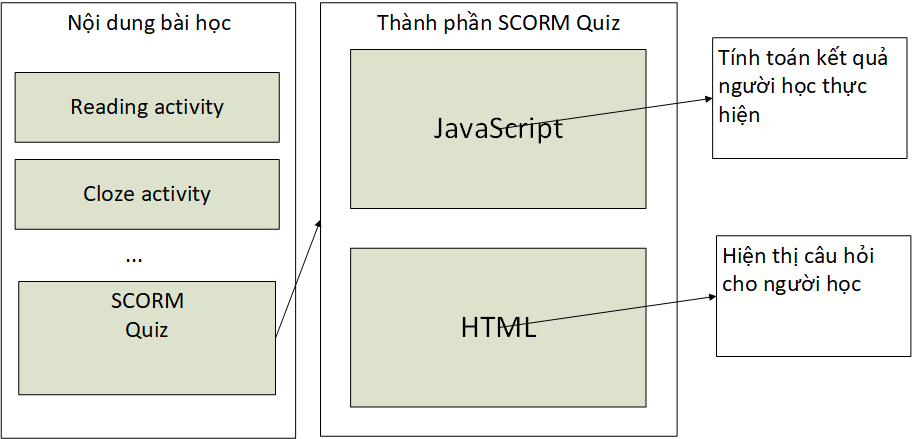
\includegraphics[width=15cm]{Chapter4/Pictures/picture41.png}
		\end{center}
		\caption{Nội dung bài học và thành phần của SCORM Quiz}
		\label{refpicture51}
	\end{figure}
\end{center}

Như vậy hình 4.1 đã cho ta thấy hạn chế của SCORM Quiz nằm ở chỗ mỗi SCORM Quiz chỉ đẩy ra được một kết quả và bộ tính toán kết quả chỉ nhận được một kết quả đưa vào. \\

\textbf{b. Cải tiến thiết kế SCORM Quiz}\\

	Để khắc phục vấn đề nêu trên, cần cải tiến mội số thiết kế của SCORM Quiz hiện tại như sau:
	\begin{itemize}
		\item Cần có một định danh duy nhất cho mỗi SCORM Quiz để các đoạn mã Javascript sau không ghi đè lên các đoạn JavaScript trước.
		
		\item Cần có một bộ tổng hợp kết quả, nhận thông tin về thiết lập của người soạn thảo rằng SCORM Quiz nào cần phải đạt.
	\end{itemize}

	\begin{center}
	\begin{figure}[htp]
		\begin{center}
			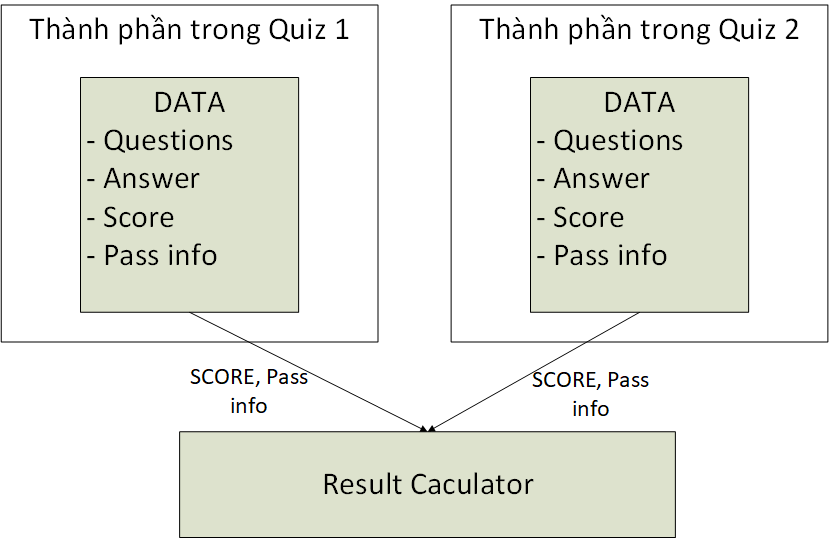
\includegraphics[width=10cm]{Chapter4/Pictures/picture42.png}
		\end{center}
		\caption{Cách cải tiến SCORM Quiz}
		\label{refpicture51}
	\end{figure}
\end{center}	

Hình 4.2 là mô hình SCORM Quiz cải tiến được đề xuất và hiện thực. Khắc phục được hạn chế về số lượng các SCORM Quiz trong một nội dung bài học như trước. Hiện thực một bộ tổng hợp kết quả gồm các toán tử logic với đầu vào là kết quả từ các SCORM Quiz có trong bài học của cây học tập và thông tin về những SCORM Quiz được người biên soạn đặt giá trị cần phải đạt, đầu ra sẽ đưa vào LMS để xử lý.

	\begin{center}
	\begin{figure}[htp]
		\begin{center}
			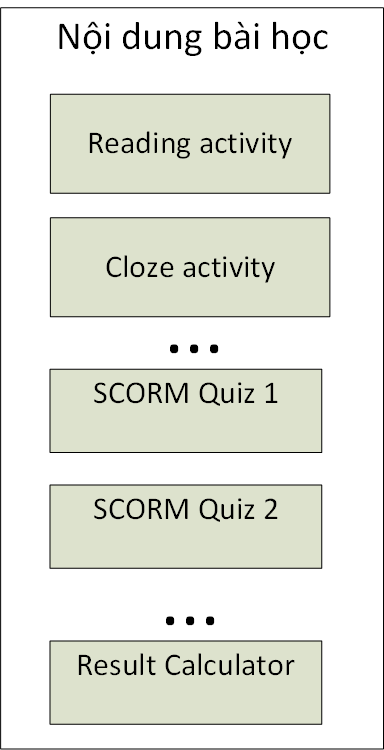
\includegraphics[width=7cm]{Chapter4/Pictures/picture43.png}
		\end{center}
		\caption{Thứ tự bộ Total score Caculator nằm trong resource file}
		\label{refpicture51}
	\end{figure}
\end{center}

	Như đã trình bày mỗi SCORM Quiz là một hoạt động được soạn thảo ra từ chức năng soạn thảo SCORM Quiz. Nội dung SCORM Quiz này sẽ bao gồm hai thành phần chính là mã Javascript để thực thi các phương thức lấy kết quả do người học lựa chọn và tính toàn điểm số, thành phần thứ hai là mã HTML để tạo ra các khung nhìn về câu hỏi cho người học thực hiện. \\
	
	Khi có nhiều SCORM Quiz được thiết kế thì sẽ có nhiều khối tương ứng được sinh ra như trong hình 4.3. Bộ tổng hợp kết quả cũng là một khối nhưng chỉ gồm một thành phần mà mã Javascript chứa các phương thức tổng hợp dành cho các SCORM Quiz. Hình 4.3 mô tả thứ tự tạo ra của các khối trong tập tin mã nguồn. Khối này sẽ được tạo ra sau SCORM Quiz cuối cùng. Như vậy LMS sẽ không nhận kết quả từ các SCORM Quiz ban đầu nữa mà chỉ nhận kết quả từ đây.\\


\subsection{Mở rộng thuộc tính cho SCORM Quiz}

	Các câu hỏi được soạn thảo trên SCORM Quiz của eXe Learning khi người biên soạn xem lại sẽ gây ra rất nhiều khó khăn. Khó khăn thứ nhất là không phân biệt được câu hỏi này thuộc phần nào trong bài học, thiếu thuộc tính phân loại về chủ đề. Khó khăn thứ hai không phân loại được độ khó của câu hỏi, thiếu thuộc tính phân loại về độ khó. Khó khăn lớn nhất là không thể tổng hợp các câu hỏi từ nhiều SCORM Quiz và tiến hành lựa chọn để tổng hợp thành một bài kiểm tra gồm nhiều mức độ và thể loại khác nhau.\\
	
	Các thuộc tính phân loại câu hỏi là cần thiết trong quá trình soạn thảo, đánh giá và tổng hợp một bài kiểm tra. Do đó, phần này sẽ đi sâu vào nghiên cứu và tìm cách khắc phục khuyết điểm này của SCORM Quiz bằng cách thêm thuộc tính phân loại vào quá trình soạn thảo.\\
	
	Về mặt thiết kế của SCORM Quiz bao gồm:
	\begin{itemize}
		\item Instructions: Các hướng dẫn sử dụng khi người biên soạn mở chức năng này.
		
		\item Question Text Area: Vùng để người biên soạn nhập câu hỏi.
		
		\item Options: Vùng nhập các câu trả lời cho câu hỏi.
		
		\item Correct Answer: Đáp án đúng của câu hỏi.
		
		\item User Answer: Đáp án người học lựa chọn.
	\end{itemize}
	
Ta sẽ thêm 3 thuộc tính về độ khó như sau: isHard, isMedium, isEasy có kiểu dữ liệu là Boolean để lưu trữ độ khó của câu hỏi này khi người soạn thảo soạn xong như hình 4.4 mô tả.	


	\begin{center}
	\begin{figure}[htp]
		\begin{center}
			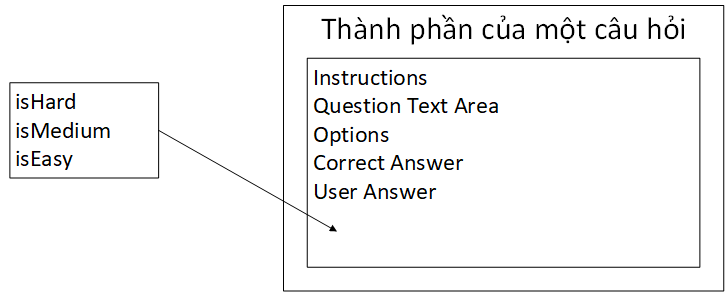
\includegraphics[width=15cm]{Chapter4/Pictures/picture44.png}
		\end{center}
		\caption{Thêm ba thuộc tính phân loại vào các các thành phần của một câu hỏi}
		\label{refpicture51}
	\end{figure}
\end{center}

Về mặt hiển thị đối với người biên soạn. Ba thuộc tính trên sẽ được biểu diễn bằng nhóm các đối tượng radio button. Bao gồm 3 radio button Hard (Khó), Medium (Trung bình) và Easy (Dễ) như hình 4.5 mô tả.

\newpage
	\begin{center}
	\begin{figure}[htp]
		\begin{center}
			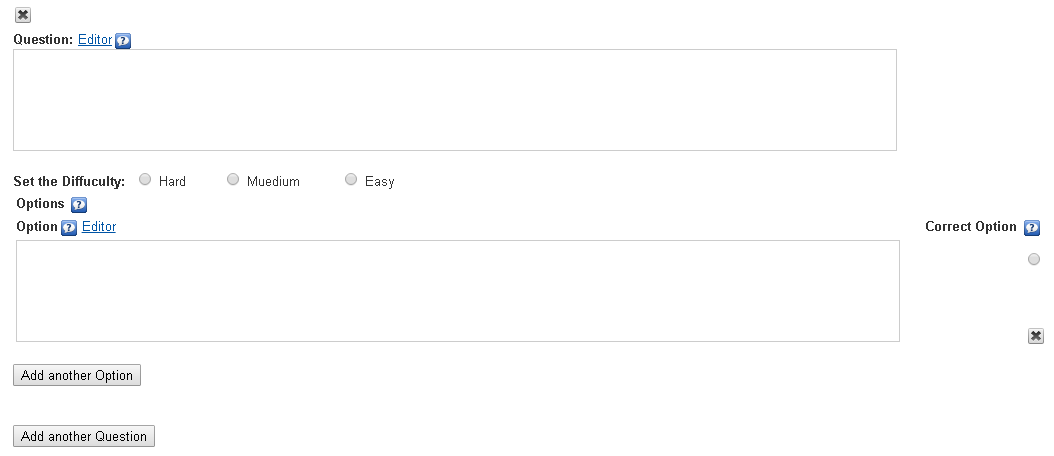
\includegraphics[width=15cm]{Chapter4/Pictures/picture45.png}
		\end{center}
		\caption{Giao diện soạn thảo câu hỏi}
		\label{refpicture51}
	\end{figure}
\end{center}


	Thuộc tính độ khó này đóng vai trò rất quan trọng trong quá trình soạn thảo bài học. Thuộc tính phân loại giúp người soạn thảo đánh giá được mức độ của bài học. Kiểm soát được mức độ của bài học cũng như mức độ của SCORM Quiz. Các thuộc tính độ khó này chỉ xuất hiện ở khung nhìn của người soạn thảo như hình 4.6, người học sẽ không thấy được thuộc tính này, có nghĩa là người học sẽ không biết được câu hỏi mình đang thực hiện có độ khó như thế nào.
	
	
	\begin{center}
		\begin{figure}[htp]
			\begin{center}
			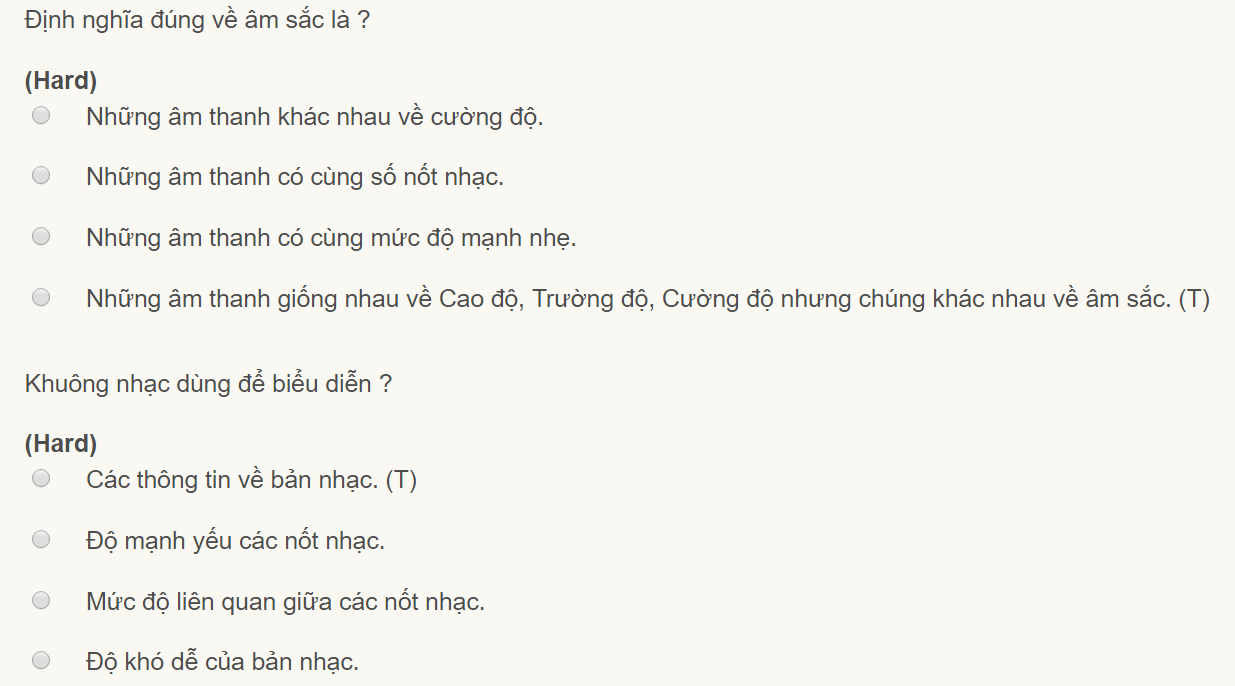
\includegraphics[width=15cm]{Chapter4/Pictures/picture46.png}
			\end{center}
			\caption{Ví dụ một khung nhìn của người soạn thảo}
			\label{refpicture52}
		\end{figure}
	\end{center}	

	\newpage
		
	\subsection{Chức năng tổng hợp câu hỏi và tạo bài kiểm tra}
	\textbf{a.	Tổng hợp câu hỏi}\\
	
		Soạn thảo câu hỏi, đánh giá người học dựa trên các câu hỏi của một SCORM Quiz không thì vẫn chưa đủ. Vì mỗi SCORM Quiz thường được biên soạn với mục đích ôn tập kiến thức là chủ yếu. Mỗi SCORM Quiz thường xoay quanh một chủ đề nhất định, không bao quát được tất cả vấn đề trong bài học. SCORM Quiz thường có số lượng câu hỏi ít từ năm đến mười câu hỏi, vì nếu soạn thảo nhiều câu hỏi trên giao diện soạn thảo của SCORM Quiz sẽ rất khó khăn do độ trễ của mỗi thao tác càng lúc càng lớn.\\
		
		Do thiết kế cứng nhắc ban đầu của SCORM Quiz nên nội dung các câu hỏi của SCORM Quiz được tạo cho người học thực hiện là cố định, không có sự thay đổi của số câu hỏi cũng như vị trí câu hỏi và câu trả lời. Hình 4.7 là mô tả việc xuất nội dung của SCORM Quiz thành resource file. Resource file này sẽ gồm hai phần chính là mã Javascript ghi nhận các câu trả lời mà người học chọn và tính điểm, phần câu hỏi và các lựa chọn trả lời sẽ được hiển thị dưới dạng HTML cứng không thay đổi được với các lần truy cập khác nhau, dẫn đến việc không khách quan nếu như người học làm lại lần thứ hai, lần thứ ba,...\\
	
	\begin{center}
	\begin{figure}[htp]
		\begin{center}
			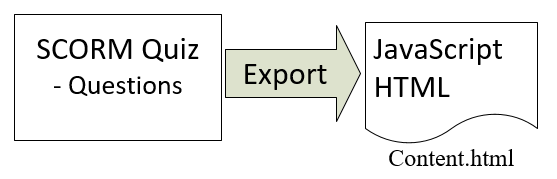
\includegraphics[width=10cm]{Chapter4/Pictures/picture47.png}
		\end{center}
		\caption{SCORM Quiz xuất nội dung thành Resource File}
		\label{refpicture55}
	\end{figure}
\end{center}
	
	Để khắc phục các hạn chế trên, nhóm đề xuất hiện thực một chức năng soạn thảo, tổng hợp câu hỏi từ nhiều SCORM Quiz dựa trên độ khó của mỗi câu hỏi. Các câu hỏi được tạo cho người học sẽ thay đổi được vị trí cũng như vị trí câu trả lời trong từng câu hỏi. Chức năng này được thiết kế thành một công cụ kiểm tra riêng biệt với tên SCORM Test.\\
	
	SCORM Test là một chức năng sẽ được xây dựng sẵn trong hệ thống eXe Learning. Được lưu trữ trong iDevice Store cùng với các iDevice khác. iDevice Store này sẽ được lưu trữ Local trong thiết bị. Được thiết kế như là một chức năng soạn thảo câu hỏi tương tự như SCORM Quiz nhưng đi kèm một số tính năng vượt trội hơn.\\
	
	iDevice này sẽ có 3 chế độ hoạt động khác nhau. Edit Mode, Author View Mode và Learner View Mode. Edit Mode là chế độ soạn thảo cho người biên soạn. Author View Mode là chế độ xem dành cho người soạn thảo, giống như SCORM Quiz, soạn thảo xong sẽ chuyển sang chế độ này. Learner View Mode là chế độ xem dành cho người học, khác với Author View Mode, chế độ xem này chỉ có những câu hỏi nào người biên soạn chọn mới được đưa ra ở đây.

	\begin{center}
	\begin{figure}[htp]
		\begin{center}
			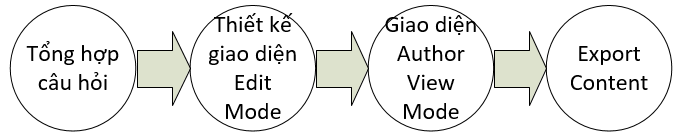
\includegraphics[width=10cm]{Chapter4/Pictures/picture48.png}
		\end{center}
		\caption{Quy trình hiện thực công cụ kiểm tra SCORM Test}
		\label{refpicture56}
	\end{figure}
\end{center}

	
\newpage

	Hình 4.8 là mô tả quá trình nhóm hiện thực iDevice. Bước đầu là việc thiết kế giao diện tổng hợp các câu hỏi từ các SCORM Quiz. Thiết kế bộ Selector để cho người biên soạn lựa chọn câu hỏi xuất hiện trong bài kiểm tra. Tiếp theo là thiết kế giao diện hiển thị cho người soạn thảo, giao diện này sẽ khác so với giao diện làm câu hỏi của người học. Cuối cùng là hiện thực phần xuất các thành phần của iDevice  thành Resource file. Resource file này phải khắc phục được các hạn chế của SCORM Quiz trình bày ra ở hình 4.1, phải đảm bảo sao cho các câu hỏi mỗi lần thực hiện trên SCORM Cloud phải là động.\\
	
		
	\textbf{b. Hiện thực việc thiết kế iDevice}\\
	
	SCORM Test là iDevice dùng cho việc soạn thảo và tổng hợp. Do đó, có tích hợp cả tính năng soạn thảo câu hỏi của SCORM Quiz vào, người dùng có thể sử dụng SCORM Test để soạn thảo câu hỏi. Tuy nhiên nhiệm vụ và chức năng chính của SCORM Test là tổng hợp câu hỏi và lựa chọn câu hỏi từ nhiều SCORM Quiz khác nhau. \\
	
	Từ hình 4.8 mô tả trên, nhóm đã nghiên cứu và đưa ra mô hình thiết kế tổng quan của SCORM Test như sau:
	
	\begin{center}
	\begin{figure}[htp]
		\begin{center}
			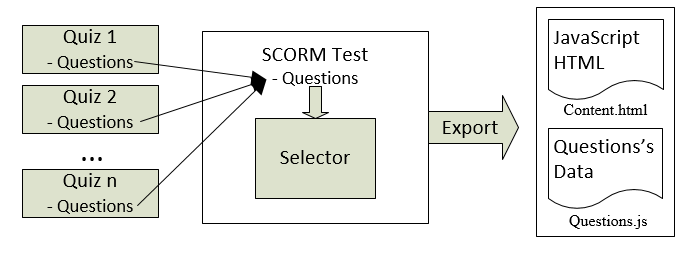
\includegraphics[width=16cm]{Chapter4/Pictures/picture49.png}
		\end{center}
		\caption{Tổ chức của SCORM Test}
		\label{refpicture57}
	\end{figure}
\end{center}

	Hình 4.9 là tổ chức của SCORM Test do nhóm đề xuất hiện thực. Mô hình này có thể khắc phục được hạn chế trong quá trình Export của SCORM Quiz. Cụ thể tất cả các bước hiện thực được đưa ra ở hình 4.9. Các bước thực gồm bốn phần được trình bày như sau.\\
	
	Phần thứ nhất, chức năng tổng hợp của SCORM Test được thực hiện như sau. Khi người dùng chọn iDevice SCORM Test, sẽ thực hiện một quá trình duyệt đệ quy trên tất các các bài học của cây học tập, quá trình này sẽ thu thập tất cả các câu hỏi từ những SCORM Quiz đã biên soạn trước được tổng hợp vào danh sách câu hỏi của SCORM Test này và hiển thị dưới dạng Edit mode cho người biên soạn chỉnh sửa. \\
	
	Phần thứ hai, chức năng lựa chọn câu hỏi được thực hiện như sau. Sau khi quá trình tổng hợp hoàn tất, sẽ xuất hiện một bộ Selector ở dưới phần câu hỏi. Bộ Selector này sẽ gồm ba trường nhập vào cho mỗi SCORM Quiz tương ứng với ba mức độ câu hỏi khó, trung bình và dễ. Người biên soạn sẽ nhập vào số lượng câu hỏi tương ứng.

\newpage

	\begin{center}
	\begin{figure}[htp]
		\begin{center}
			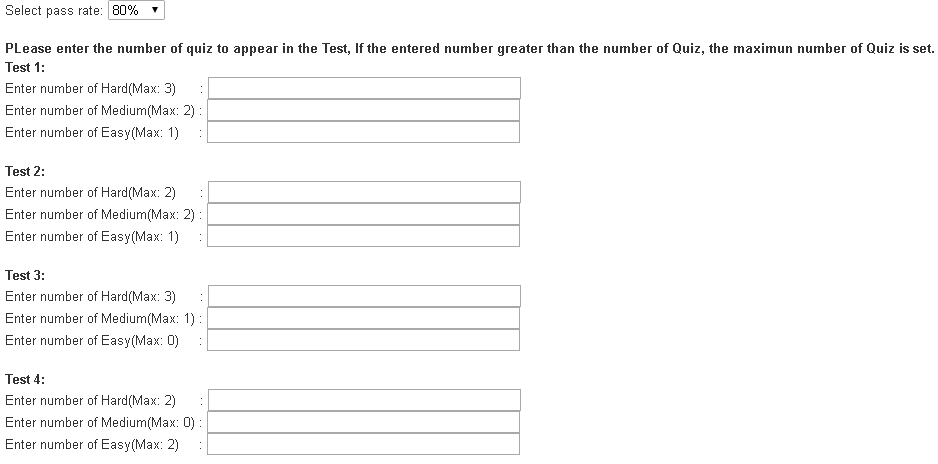
\includegraphics[width=16cm]{Chapter4/Pictures/picture410.png}
		\end{center}
		\caption{Chế độ Edit Mode của SCORM Test}
		\label{refpicture58}
	\end{figure}
\end{center}

Hình 4.10 là giao diện cho bộ cấu hình bài kiểm tra của SCORM Test. Người soạn thảo sẽ lựa chọn tỷ lệ đạt (Pass Rate) cho bài kiểm tra và chọn các câu hỏi sẽ được hiển thị lên bài kiểm tra. Số câu hỏi tối đa của từng độ khó cũng sẽ được thống kê ở đây, nếu người dùng nhập vào số lượng câu hỏi nhiều hơn số câu hỏi tối đa thì số câu hỏi tối đa sẽ được chọn.\\

	\begin{center}
	\begin{figure}[htp]
		\begin{center}
			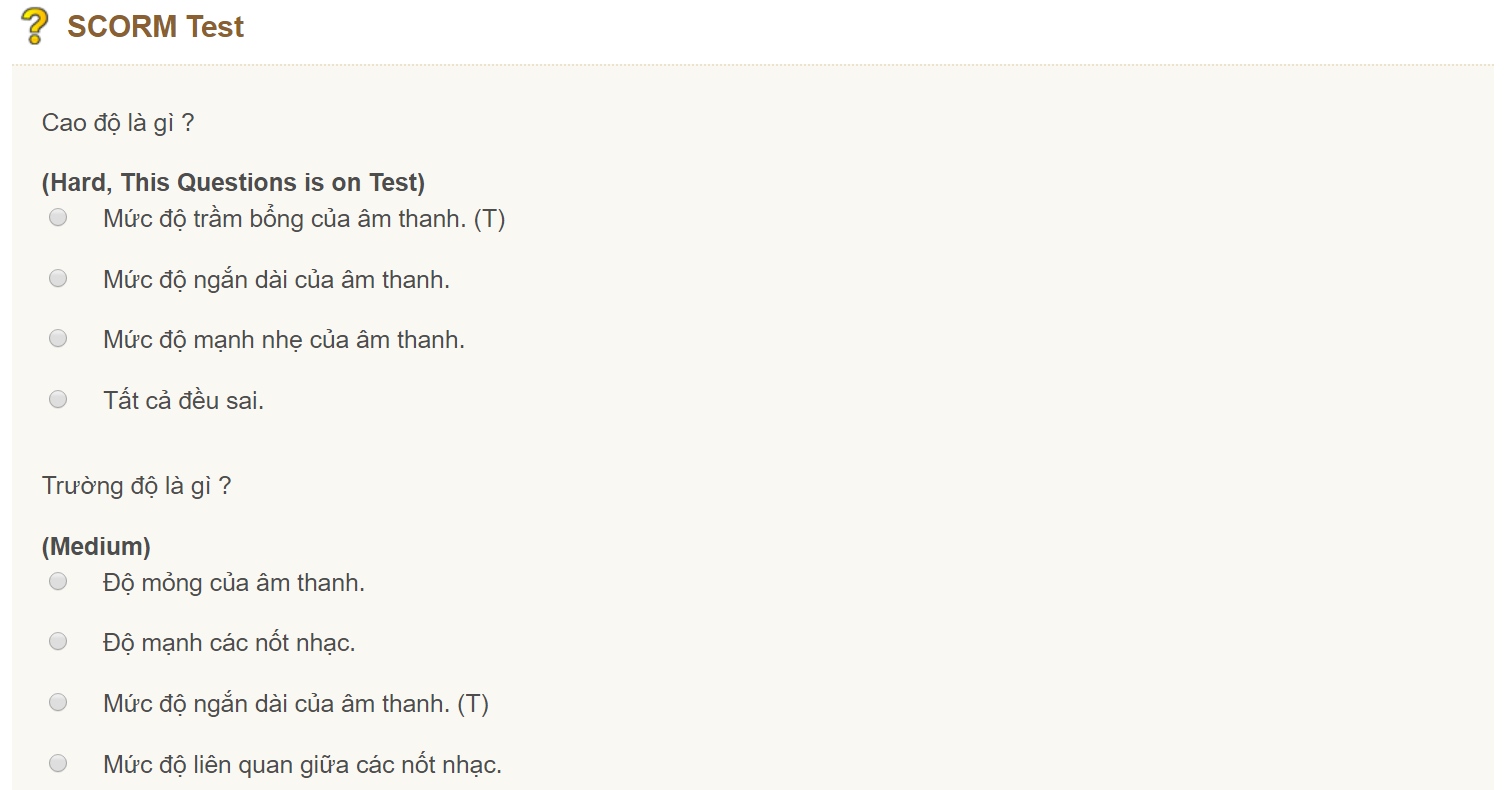
\includegraphics[width=16cm]{Chapter4/Pictures/picture411.png}
		\end{center}
		\caption{SCORM Test ở chế độ Author View Mode}
		\label{refpicture58}
	\end{figure}
\end{center}

\newpage

	Phần thứ ba, sau khi người soạn thảo cấu hình xong sẽ chuyển sang View mode dành cho người biên soạn. Người biên soạn có thể theo dõi được tất cả các câu hỏi có trong bài học. Hình 4.11 là giao diện Author View Mode. Các câu hỏi sẽ được gắn hai nhãn đánh dấu, nhãn thứ nhất đánh dấu về độ khó của câu hỏi, nhãn thứ hai đánh dấu cho biết câu hỏi nào sẽ được xuất hiện trong bài kiểm tra.\\
	
	Phần thứ tư là xuất các nội dung đã được thiết lập trong quá trình soạn thảo SCORM Test thành các Resource File. Đây là bước khó nhất trong toàn bộ quá trình đã đưa ra ở hình 4.9, phải nghiên cứu và khắc phục được mô hình Export cứng nhắc của SCORM Quiz. Nhóm đề xuất một quá trình Export thành hai file khác nhau, Một file data chứa nội dung các câu hỏi và trả lời tương ứng định với dịnh dạng file Javascript. File thứ hai là file chứa nội dung của bài học theo định dạng file HTML. \\
	
	File nội dung định dạng HTML này sẽ gồm hai phần, phần đầu sẽ là mã JavaScript, phần thứ 2 là mã HTML chứa nội dung được hiển thị ra. Nguyên tắc xử lý sẽ được trình bày như sau.\\
	
		\begin{center}
		\begin{figure}[htp]
			\begin{center}
				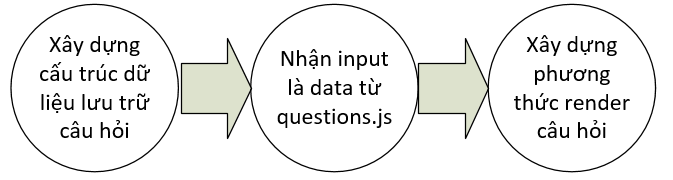
\includegraphics[width=15cm]{Chapter4/Pictures/picture412.png}
			\end{center}
			\caption{Công việc của mả Javascript trong file content.html}
			\label{refpicture510}
		\end{figure}
	\end{center}


Hình 4.12 mô tả quá trình hiện thực mã Javascript trong file content.html. Bước thứ nhất sẽ xây dựng một cấu trúc dữ liệu thích hợp dùng để lưu trữ câu hỏi, một câu hỏi sẽ có các thuộc tính được định nghĩa như bảng 4.1 ở dưới.\\

\begin{table}[!htp]
	\centering
	\begin{tabular}{|l|c|l|}
		\hline 
		\textbf{Name} 	& \textbf{Data Type} 	& \hspace{2.6cm}\textbf{Ý nghĩa} \\ 
		\hline 
		Id 				& String 				& Định danh duy nhất cho từng câu hỏi.\\ 
		\hline 
		Text 			& String 				& Phần nội dung câu hỏi.\\ 
		\hline 
		Answers 		& Array 				& Mảng chứa các câu trả lời tương ứng.\\ 
		\hline 
		CorrectAnswer	& String 				& Câu trả lời đúng.\\ 
		\hline
		ObjectID 		& String 				& Cho biết câu hỏi này thuộc Object nào.\\  
		\hline
	\end{tabular}
	\caption{Các thuộc tính của một câu hỏi}
	\label{reftable51}
\end{table}

%Bước thứ hai sẽ nhận input là data từ file questions.js để đọc và lưu trữ thành một mảng các Questions Object. File questions.js là phần đầu của Resource File như đã trình bày ở trên. Mảng các Questions Object là mảng chứa các câu hỏi đã lưu trữ, với mục đích tạo bài kiểm tra.\\

Bước thứ hai, sẽ nhận input là data từ file questions.js để đọc và lưu trữ thành một mảng các Questions Object.\\

		\begin{center}
	\begin{figure}[htp]
		\begin{center}
			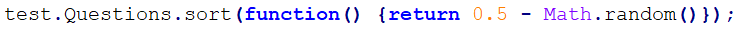
\includegraphics[width=15cm]{Chapter4/Pictures/picture413.png}
		\end{center}
		\caption{Đoạn mã Javascript sắp xếp lại các câu hỏi ở mỗi lần tạo}
		\label{refpicture510}
	\end{figure}
\end{center}

Bước thứ ba là xây dựng các phương thức sinh bài kiểm tra với khung nhìn của người học từ mảng câu hỏi đã được lưu trữ. Mỗi lần tạo sẽ thực hiện việc sắp xếp lại thứ tự các câu hỏi trong mảng bằng cách sử dụng hàm sort có sẵn trong Javascript, hình 4.13 mô tả đoạn mã này, với mục đích đảm bảo rằng các câu hỏi ở mỗi lần hiển thị đều sẽ ở các vị trí khác nhau.



\subsubsection{c. Kết quả}

Kiểm tra kết quả sau khi hiện thực được tiến hành như sau. Sau khi hiện thực thành công chức năng, tiến hành đóng gói nội dung với nhiều SCORM Quiz, ở bài học cuối cùng ta dùng tính năng SCORM Test để tổng hợp câu hỏi, đóng gói nội dung lại và upload lên SCORM Cloud để kiểm tra kết quả. Hình 4.14 là giao diện khóa học khi upload nội dung lên SCORM Cloud.

	\begin{center}
		\begin{figure}[htp]
			\begin{center}
				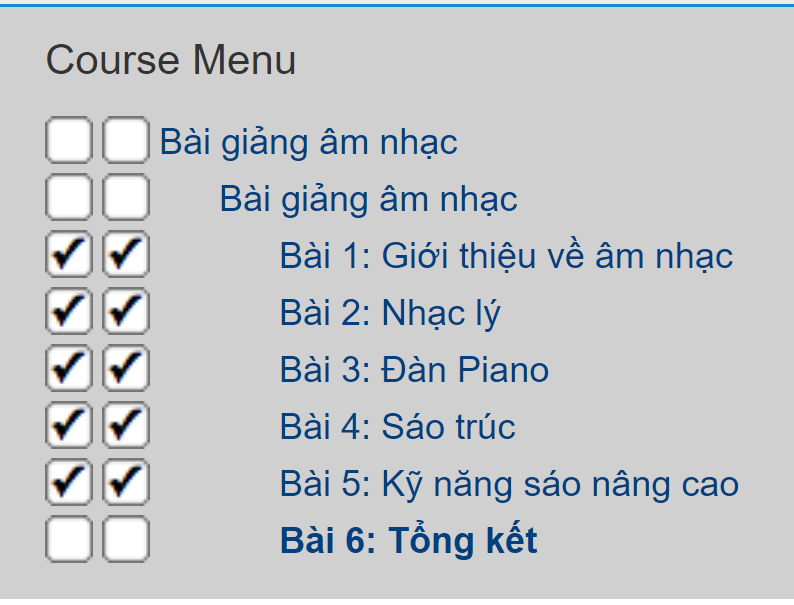
\includegraphics[width=9cm]{Chapter4/Pictures/picture414.png}
			\end{center}
			\caption{Course menu với SCORM Test}
			\label{refpicture511}
		\end{figure}
	\end{center}

Hình 4.15 mô tả quá trình hai lần thực hiện SCORM Test. Ta có thể thấy các câu hỏi cũng như các câu trả lời tương ứng đã có thể thay đổi được vị trí khi thực hiện nhiều lần khác nhau.

	\begin{center}
		\begin{figure}[htp]
			\begin{center}
				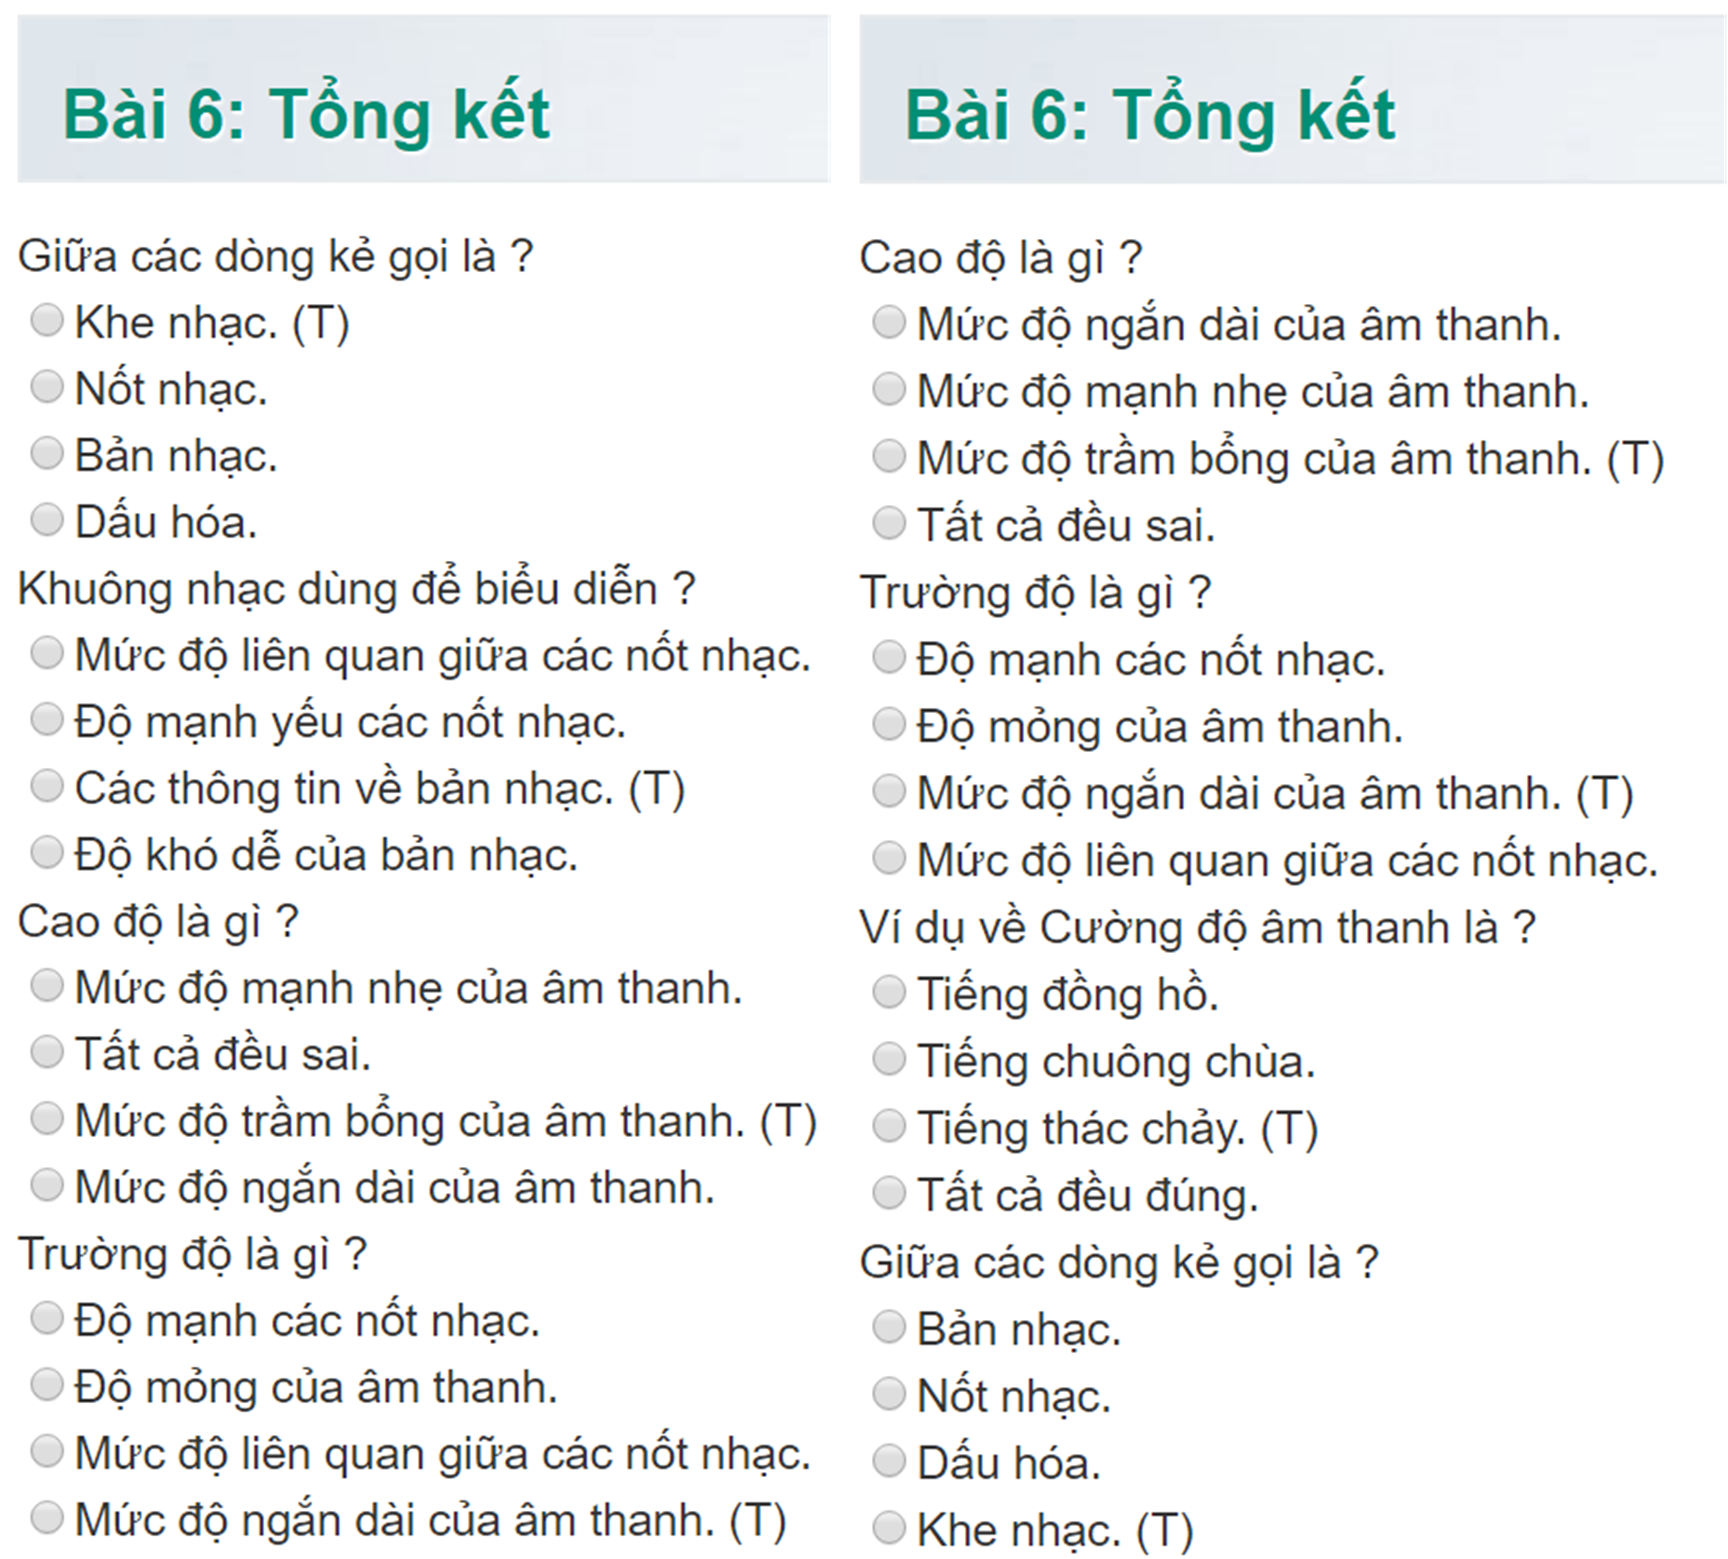
\includegraphics[width=10cm]{Chapter4/Pictures/picture415.png}
			\end{center}
			\caption{Sinh đề kiểm tra với SCORM Test }
			\label{refpicture512}
		\end{figure}
	\end{center}







